\newpage
\section{\label{intro_extrap}Introduction} 

The OpenExtrap software contains programs which makes use of a recursive extrapolation algorithm in the space-frequency domain.  The total package consists of 5 related programs. 
Each program gets its parameters from the command-line according to the SU convention. 
Not all parameters have to be specified. 
For most parameters the default values should be sufficient. 
All parameters are explained in separate sections, discussing the individual programs.

The extrapolation in the space-frequency domain is performed with optimized spatial convolution operators. 
Default are the Weighted Least Squares operators (WLSQ) which are described in Thorbecke (2004).
Note that the optimized extrapolation operators are the columns($\boldmath W^+$) and rows($\boldmath W^-$) of the $\boldmath W$ matrices in the $\boldmath W^- \boldmath R^+ \boldmath W^+$ model. 

The programs in the package all have the same structure. 
This structure is also reflected in the filenames of the different functions. 
In the initial stage of the program the data to be extrapolated (wave field measurements) and the gridded medium files (velocity and density) are read in . 
From the velocity file the minimum and maximum velocity is determined and together with the desired minimum and maximum frequency an operator table is calculated in advance. 
The operator table is stored in memory as an static array (see the {\bf tablecalc$\dots$.c} functions). 

The {\bf xw$\dots$.c} functions perform the extrapolation and calculate the specific results. 
In these {\bf xw$\dots$.c} functions the data is transformed to the space-frequency domain and for every lateral position, for all depth steps and for all frequencies, a convolution is carried out with the optimized convolution operator. 
Note that a new convolution operator is read from the table if the wavenumber $k$ changes, so if the velocity or frequency changes.
After the extrapolation has finisched the calculated result is transformed to the space-time domain and the function returns to the main program.

In the sub-directory {\it main} the following programs can be found:

\begin{itemize}
\item
\htmlref{{\bf extrap}}{extrap} - extrapolation through a gridded subsurface model.
\item
\htmlref{{\bf cfpmod}}{cfpmod} - modeling one-way travel times for CFP operator generation.
\item
\htmlref{{\bf migr}}{migr} - shot record migration using optimized extrapolation operators.
\item
\htmlref{{\bf migr\_mpi}}{migr} - parallel shot record migration using optimized extrapolation operators.
\item
\htmlref{{\bf opercalc}}{opercalc} - calculates extrapolation operators for a given frequency.
\item
\htmlref{{\bf onewvsp}}{onewvsp} - VSP generation with one-way extrapolation operators.
\end{itemize}

In the sub-directory {\it lib} there are two types of functions defined; functions which are related to the calculation of different optimized convolution operators, and functions which are related to the calculation of the spatial convolution.

\begin{tabular} {| p{2.2cm} | p{9cm} |}
\hline {\bf operator} & GaussWindow, KaiserWindow, forwExtr, invExtr, kxwfilter, optRemez, remez, shortoper, spline3,
tablecalc\_opt, trunc1D, weightfunct, toeplitz, findBestOper \\ \hline \hline 
{\bf convolution} & xwMigrOpl, xwBeam, xwCFP, xwExtr, xwSnap, xwVSP, extrapEdge, xwZoMigr, xwExtrG, kwZoMigr, kwExtr, kwMigr \\ \hline \hline 
{\bf from SU} & atopkge, docpkge, getpars \\ \hline \hline 
{\bf misc} & calc\_vz, getreccfp, getrecvsp, minmax, srcarray, verbosepkg, getFileInfo, getModelInfo, readData, writeData,
wallclock\_time
\\ \hline
\end{tabular}
\\

The spatial convolution (for every frequency) is implemented in an efficient way by making use of the symmetry in the convolution operator. 
On a vector machine this code should work very well. 
It may be usefull to use these subroutines in other programs where an extrapolation is needed.

Further details on the individual programs are documented in the next sections. All programs are selfdocumented.

The demo directory contains a gridded velocity file {\tt syncline\_cp.su} shown and in Figure \ref{model} and a Ricker wavelet shown
in Figure \ref{wave}.
%
\begin{figure}[hb]
  \begin{pspicture}(8,7)
    \put(-0.55,-0.3){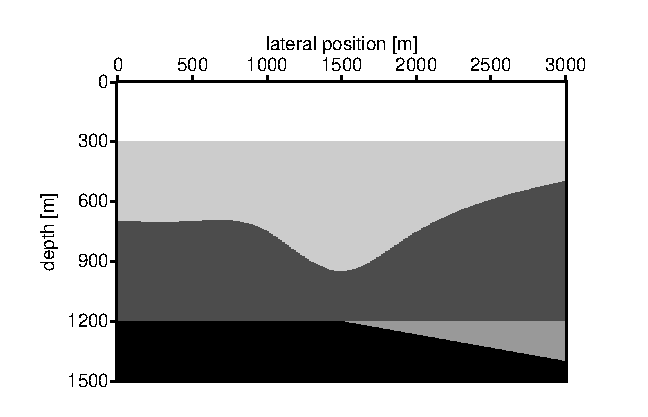
\epsfig{file=EPS/model.eps,width=12cm}}
%	\psgrid
\end{pspicture}
\caption{ Syncline model which is used in the demo directory to illustrate the working of the programs. } \label{model}
\end{figure}
%

\begin{figure}[hb]
  \begin{pspicture}(14,7)
    \put(0.0,-0.3){\epsfig{file=EPS/wave.eps}}
    \put(5.0,-0.3){\epsfig{file=EPS/wavefreq.eps}}
%	\psgrid
\end{pspicture}
\caption{ Ricker wavelet(left) and amplitude spectrum(right) which is used in the modeling experiments of the demo directoty. } \label{wave}
\end{figure}
%


